
\begin{figure*} [t!]
%\begin{tcolorbox}[colframe=black!30!black, colback=white]
\hfill
\begin{subfigure}[r]{0.5\textwidth}
    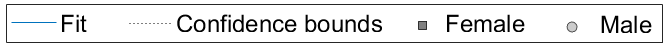
\includegraphics[width=\textwidth]{Figures/legend}
  \end{subfigure}
  \vskip\baselineskip
  \hspace{-5mm}
  \begin{subfigure}[b]{0.51\textwidth}
    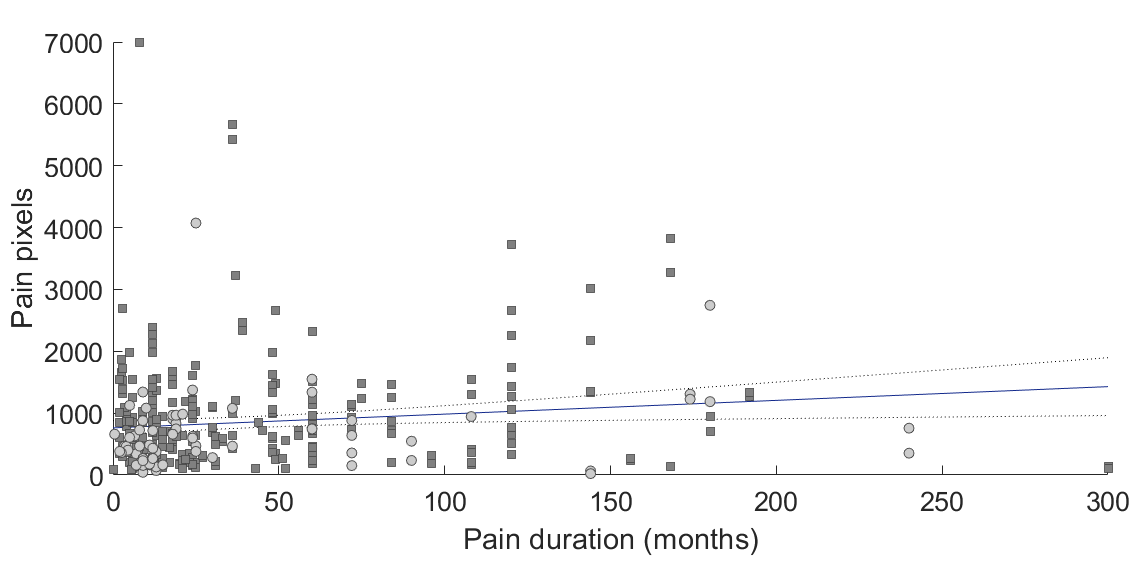
\includegraphics[width=\textwidth]{Figures/durapixel}
    \caption{ }
    \label{fig:1}
  \end{subfigure}
  \hfill
    \hspace{2mm}
  \begin{subfigure}[b]{0.51\textwidth}
    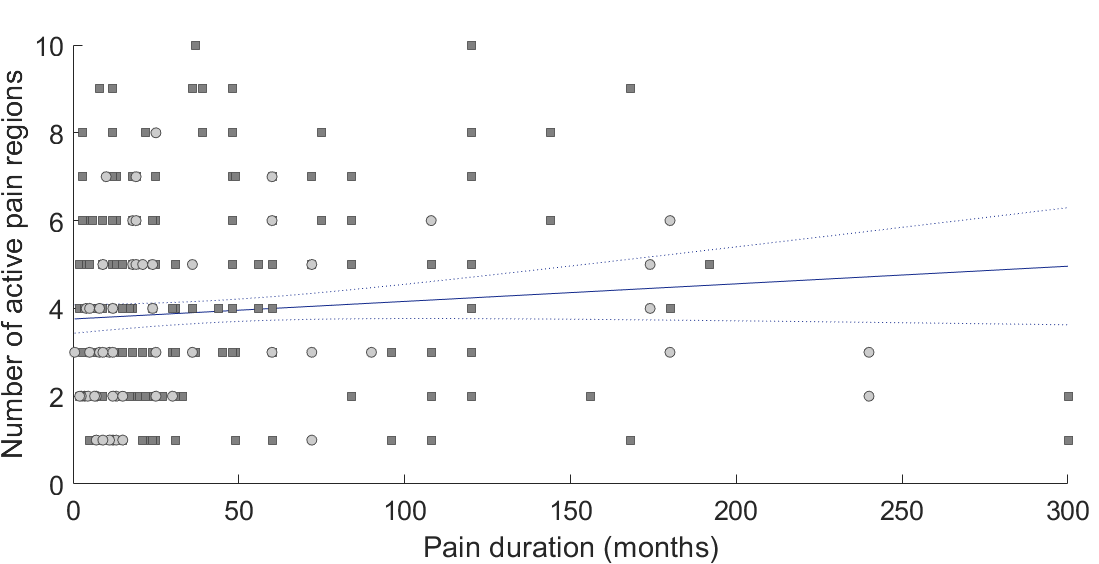
\includegraphics[width=\textwidth]{Figures/duraregion}
       \caption{ }
    \label{fig:2}
  \end{subfigure}
    \vskip\baselineskip
    \hspace{-5mm}
  \begin{subfigure}[b]{0.51\textwidth}
    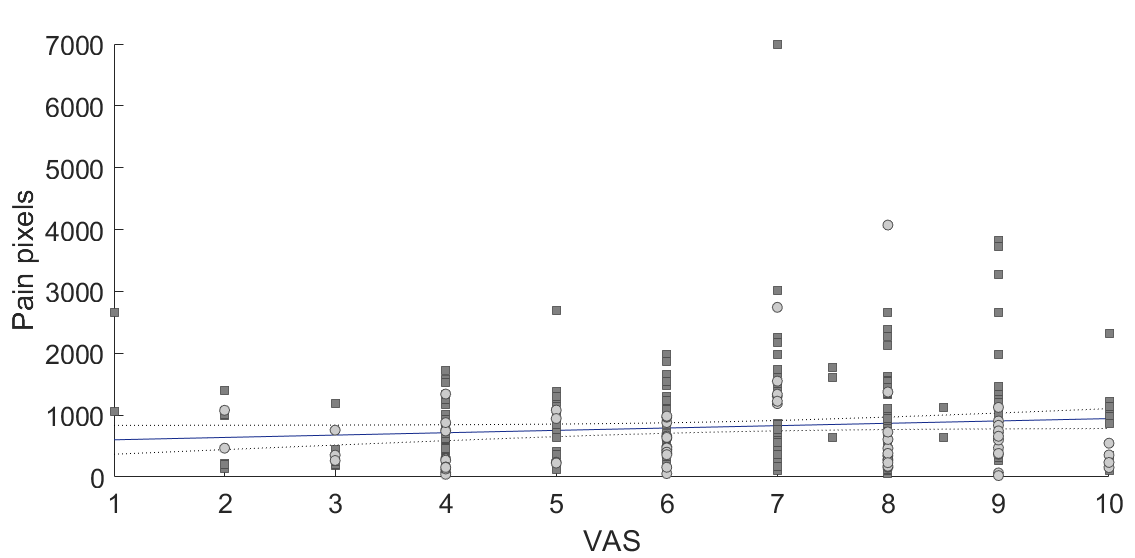
\includegraphics[width=\textwidth]{Figures/vaspixel}
    \caption{}
    \label{fig:3}
  \end{subfigure}
  \hfill
  \hspace{2mm}
  \begin{subfigure}[b]{0.51\textwidth}
    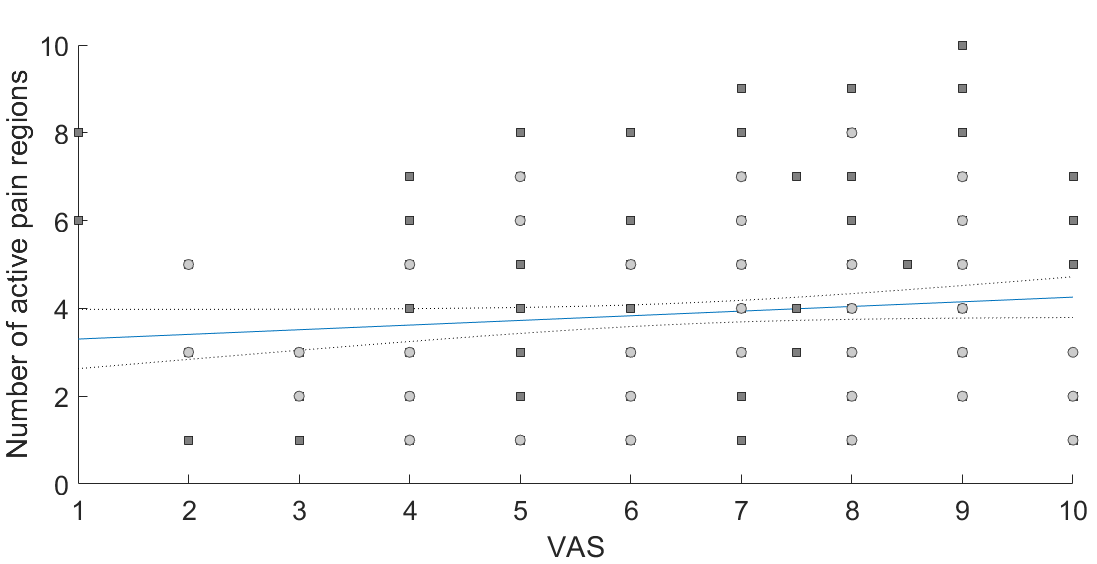
\includegraphics[width=\textwidth]{Figures/vasregion}
       \caption{ }
    \label{fig:4}
  \end{subfigure}  
  \caption{Linear correlations of pain pixels and pain duration (a), active pain regions and pain duration (b), pain pixels and pain intensity indicated in VAS (c), and active pain regions and pain intensity indicated in VAS (d).}
  \label{fig:correlations}
%\end{tcolorbox}
\end{figure*}

%\subsection{Assessment between simple features and pain duration or pain intensity} 
The linear regression between simple features, number of pain pixels or active pain regions, and pain duration or pain intensity, resulted in the plots shown in Fig. \ref{fig:correlations}. The $R^2$-values indicated a poor fit according to the linear regression lines. The regression for the correlation in Fig. \ref{fig:1} resulted in $R^2 = 0.018$, Fig. \ref{fig:2} $R^2 = 0.008$, Fig. \ref{fig:3} $R^2 = 0.011$ and Fig. \ref{fig:4} $R^2 = 0.011$. 

\begin{table*}[b!]
\centering
\begin{tabular}{@{}llll@{}}
\toprule
\multicolumn{4}{c}{\hspace{2.3cm} Accuracy (\%) \hspace{1cm} Sensitivity (\%) \hspace{1cm} Specificity (\%) \hspace{1cm}                }                                                                                                                                                                         \\ \midrule
\multicolumn{4}{c}{Morphology-representation} \\ \midrule
Pain duration  & \hspace{0.7cm}\begin{tabular}[c]{@{}l@{}}69.44\% \end{tabular} & \hspace{2.6cm} \begin{tabular}[c]{@{}l@{}}56.25\%\end{tabular} & \hspace{2.7cm} \begin{tabular}[c]{@{}l@{}} 80.00\%\end{tabular} \\ %\midrule
Pain intensity & \hspace{0.6cm} \begin{tabular}[c]{@{}l@{}}60.00\% \end{tabular}  & \hspace{2.7cm}\begin{tabular}[c]{@{}l@{}}40.00\% \end{tabular}  & \hspace{2.7cm} \begin{tabular}[c]{@{}l@{}}75.00\%\end{tabular}   \\ \midrule
\multicolumn{4}{c}{Location-representation}                                                                                                                                                                             \\ \midrule
Pain duration  & \hspace{0.6cm} \begin{tabular}[c]{@{}l@{}}35.29\%\end{tabular}  & \hspace{2.6cm} \begin{tabular}[c]{@{}l@{}}0.00\% \end{tabular}  & \hspace{2.7cm} \begin{tabular}[c]{@{}l@{}}100\%\end{tabular}  \\ %\midrule 
Pain intensity & \hspace{0.6cm} \begin{tabular}[c]{@{}l@{}}60.71\% \end{tabular}   & \hspace{2.6cm} \begin{tabular}[c]{@{}l@{}}0.00\% \end{tabular}   & \hspace{2.7cm} \begin{tabular}[c]{@{}l@{}}100\%\end{tabular}  \\ \midrule
\multicolumn{4}{c}{Combined-representation}                                                                                                                                                              \\ \midrule
Pain duration  & \hspace{0.6cm} \begin{tabular}[c]{@{}l@{}}55.56\% \end{tabular}                                                                   & \hspace{2.6cm} \begin{tabular}[c]{@{}l@{}}55.00\%\end{tabular}                                                                & \hspace{2.7cm} \begin{tabular}[c]{@{}l@{}}43.75\%\end{tabular}                                                                                                                                \\% \midrule
Pain intensity & \hspace{0.6cm} \begin{tabular}[c]{@{}l@{}}86.67\% \end{tabular}
&\hspace{2.6cm} \begin{tabular}[c]{@{}l@{}} 75.00\%\end{tabular}                                                               
& \hspace{2.7cm} \begin{tabular}[c]{@{}l@{}} 90.91\%\end{tabular}                                                               
 \\ \bottomrule
\end{tabular}
\caption{Generalization performance of the models, which use the MR, LR, and CR when classifying according to pain duration or pain intensity.}
\label{tab:performance}
\end{table*}


\begin{figure*} [b!]
%\begin{tcolorbox}[colframe=black!30!black, colback=white]
    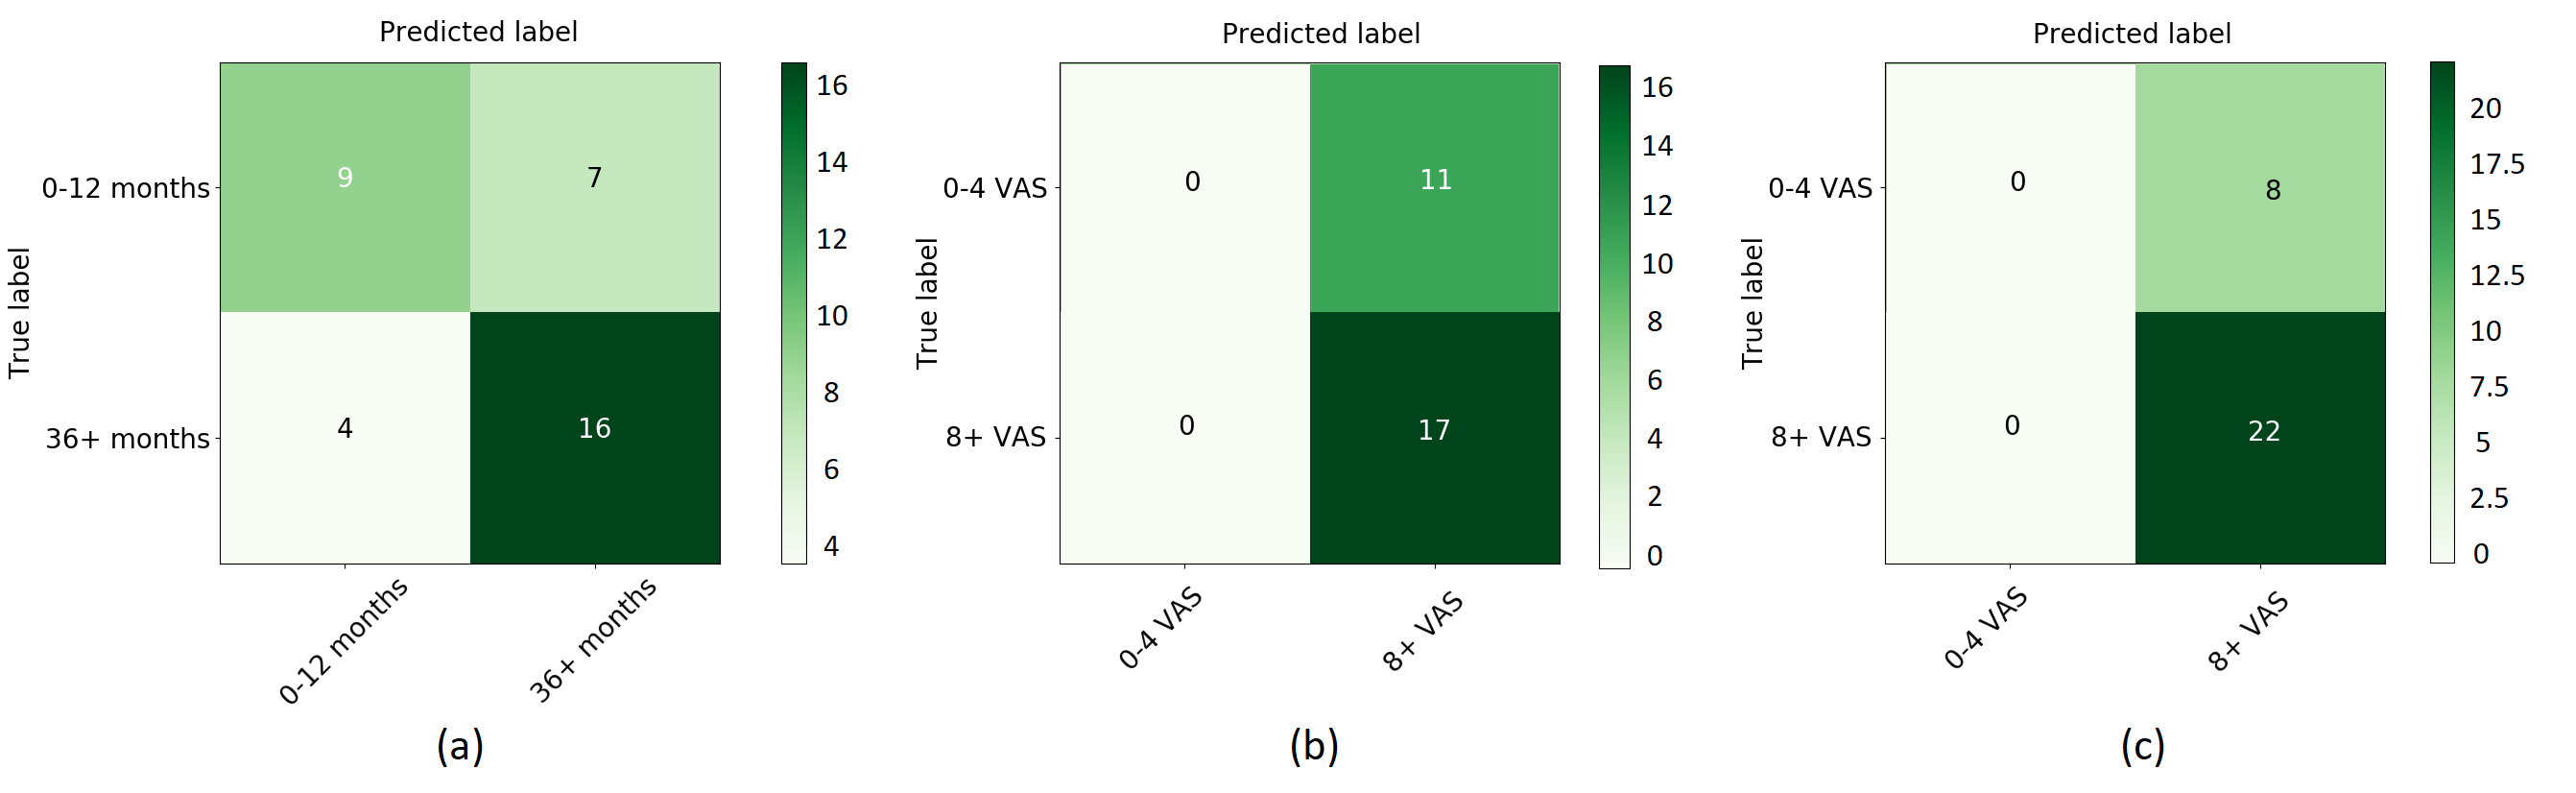
\includegraphics[width=1\textwidth]{Figures/samcon}
  \caption{Confusion matrices of (a) MR classified according to pain duration, (b) classified LR according pain duration, and (c) classified CR according to pain duration.}
  \label{fig:confma}
%\end{tcolorbox}
\end{figure*}

\begin{figure*} [t!]
%\begin{tcolorbox}[colframe=black!30!black, colback=white]
    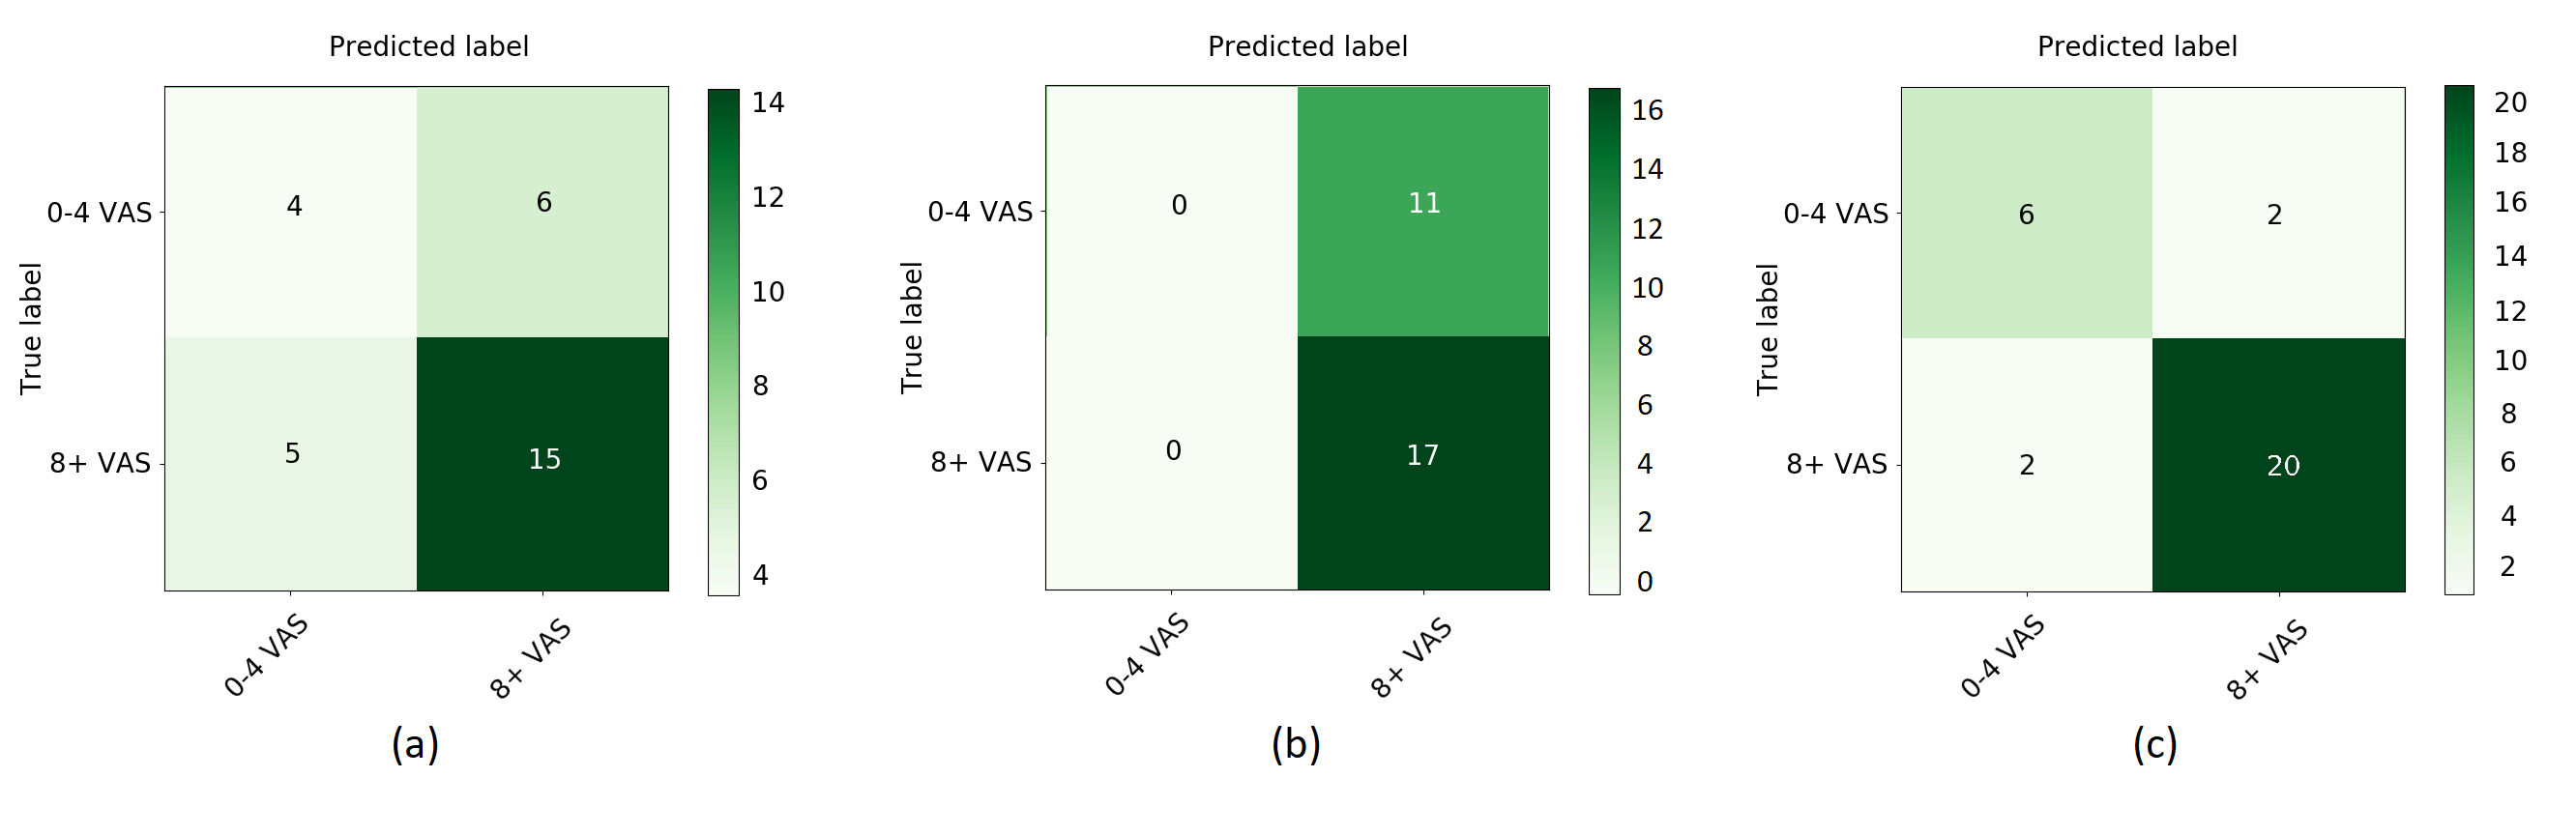
\includegraphics[width=1\textwidth]{Figures/samcon1}
  \caption{Confusion matrices of (a) MR classified according to pain intensity, (b) classified LR according pain intensity, and (c) classified CR according to pain intensity.}
  \label{fig:confma1}
%\end{tcolorbox}
\end{figure*}

\vspace{-0.3cm}
\subsection{Optimization of the models}
During the optimization, a structured grid search resulted in different hyperparameters according to each model, which is shown in Table \ref{tab:damn}.

\begin{table}[H]
\centering
\begin{tabular}{@{}llll@{}}
\toprule
                   & \begin{tabular}[c]{@{}l@{}}Learning\\ rate\end{tabular} & Nodes & \begin{tabular}[c]{@{}l@{}}Epochs/\\ Batch size\end{tabular} \\ \midrule
MR: Pain duration   & 0.01                                                    & 64    & 120/20                                                       \\
MR: Pain intensity  & 0.1                                                     & 16    & 140/10                                                       \\
LR: Pain duration   & 0.01                                                    & 16    & 120/20                                                       \\
LR: Pain intensity  & 0.01                                                    & 16    & 120/20                                                       \\
CR: Pain duration   & 0.1                                                     & 16    & 120/30                                                       \\
CR: Pain intensity  & 0.001                                                   & 16    & 120/30                                                       \\ \bottomrule
\end{tabular}
\caption{Hyperparameters chosen for each model after initial grid search.}
\label{tab:damn}
\end{table}
\noindent
For the deep learning models including MR different hyperparameters was used to obtain the highest performance. The models including the LR had similar results from the optimization. Furthermore, the model including the CR had almost identical hyperparameters except from the learning rate. 

\vspace{-0.1cm}
\subsection{Performance of the models}
The accuracy, sensitivity, and specificity of the models during test according to the representations are shown in Table \ref{tab:performance}. Furthermore, confusion matrices were created according to the pain duration as shown in Fig. \ref{fig:confma}, and confusion matrices according to pain intensity as shown in Fig. \ref{fig:confma1}.
The models that used the MR resulted in a higher predictive value for pain duration and pain intensity in the higher extremes (36-300 months and 8-10 VAS), compared to the lower extremes (0-12 months and 0-4 VAS). By comparing the sensitivity and specificity of the model using MR to predict pain duration or pain intensity, the pain duration had a higher predictive value according to the true low pain duration, and true high pain duration.
Overall, the models using the LR, could not predict according to the lower extremes, but classified only according to the higher extremes.  
The model using the CR to predict pain intensity, resulted in the best performance, based on the accuracy, sensitivity, and specificity. This model resulted similar to the models using MR, and predicted better to the higher extremes. 
The model with the highest accuracy of 86.67\% was the model using CR to predict pain intensity, whereas the lowest accuracy of 35.29\% was the model using LR predicting according to pain duration. 